\documentclass[twocolumn]{article}
\usepackage{graphicx}
\usepackage{amsmath}
\usepackage{amssymb}
\usepackage{geometry}
\usepackage{subcaption}
\usepackage{float}
\graphicspath{{./misinformation_experiment/analysis}} 


\geometry{a4paper, margin=1in}

\title{Effectiveness of Logical Rebuttal Strategies Against Misinformation: An Agent-Based Simulation Study}
\author{}
\date{\today}

\begin{document}

\maketitle

\section{Introduction}
In recent years, the spread of misinformation has emerged as a critical social, political, and public health issue. The COVID-19 pandemic notably demonstrated how misinformation about vaccine safety and false treatments can exacerbate public health crises (Roozenbeek et al., 2020). Similarly, misinformation played significant roles in deepening social and political divides, as observed in the 2020 U.S. presidential election and the Brexit referendum in the UK, undermining trust in democratic processes (Vosoughi et al., 2018).

However, misinformation cannot always be simply classified as either "true" or "false." The concept of Information Disorder provides a more nuanced framework for understanding the various forms of problematic information, distinguishing between misinformation (false information shared without intent to harm), disinformation (deliberately created and shared false information), and malinformation (genuine information shared to cause harm) (Wardle \& Derakhshan, 2017). This framework recognizes that problematic information exists on a spectrum with varying degrees of falsity and intent. Traditional fact-checking methods alone have proven inadequate for addressing these complex forms of Information Disorder. Consequently, there is a growing demand for more sophisticated strategies that specifically target different types of problematic information.

Against this backdrop, community-driven correction approaches such as Twitter's (now X's) Community Notes have attracted considerable attention. Community Notes enables users to annotate problematic content with corrective or supplemental information, allowing the community collectively to evaluate and refine the accuracy of information. However, previous research highlights that such corrections are not universally effective. Specifically, phenomena like the "Backfire Effect," wherein corrections paradoxically strengthen original false beliefs, have been documented extensively (Nyhan \& Reifler, 2010; Lewandowsky et al., 2012). Thus, the question of how to design and deliver effective corrections remains unresolved.

To address this gap, this study empirically examines the effectiveness of different rebuttal strategies proposed in the Counter-Argument Logical Structure Analysis (CALSA) framework introduced by Naito et al. (2024). This framework includes ten distinct logical strategies: Mitigation, Alternative, No Evidence, Another True Cause, Missing Mechanism (two variants), No Need to Address, Negative Effect Due to y, and Positive Effects of a Different Perspective from y (two variants). The current research evaluates the effectiveness of these strategies under various conditions to identify when and how they can most effectively counter different types of Information Disorder.

Specifically, we selected gun control as a socially significant and contentious topic and used large language models (LLMs) to generate content representing various types of Information Disorder across seven categories as defined by Wardle (2017): Satire/parody, Misleading content, False connection, False context, Imposter content, Manipulated content, and Fabricated content. We then systematically generated corresponding corrections employing the ten rebuttal strategies from the CALSA framework. To evaluate these rebuttals, we implemented two types of evaluation agents—neutral and pro-misinformation—to assess the persuasiveness and effectiveness of each type of rebuttal.

The results demonstrated clear variations in the effectiveness of rebuttal types across different categories of Information Disorder. The Missing Mechanism 2 strategy consistently showed the strongest corrective effect across multiple Information Disorder types, particularly for neutral evaluators. Conversely, the Negative Effect due to y strategy often polarized responses, receiving high ratings from neutral evaluators but low ratings from those predisposed to accept problematic information. Interestingly, certain strategies like Missing Mechanism 1 demonstrated minimal polarization, suggesting their potential utility for addressing diverse audiences.

\begin{figure*}
    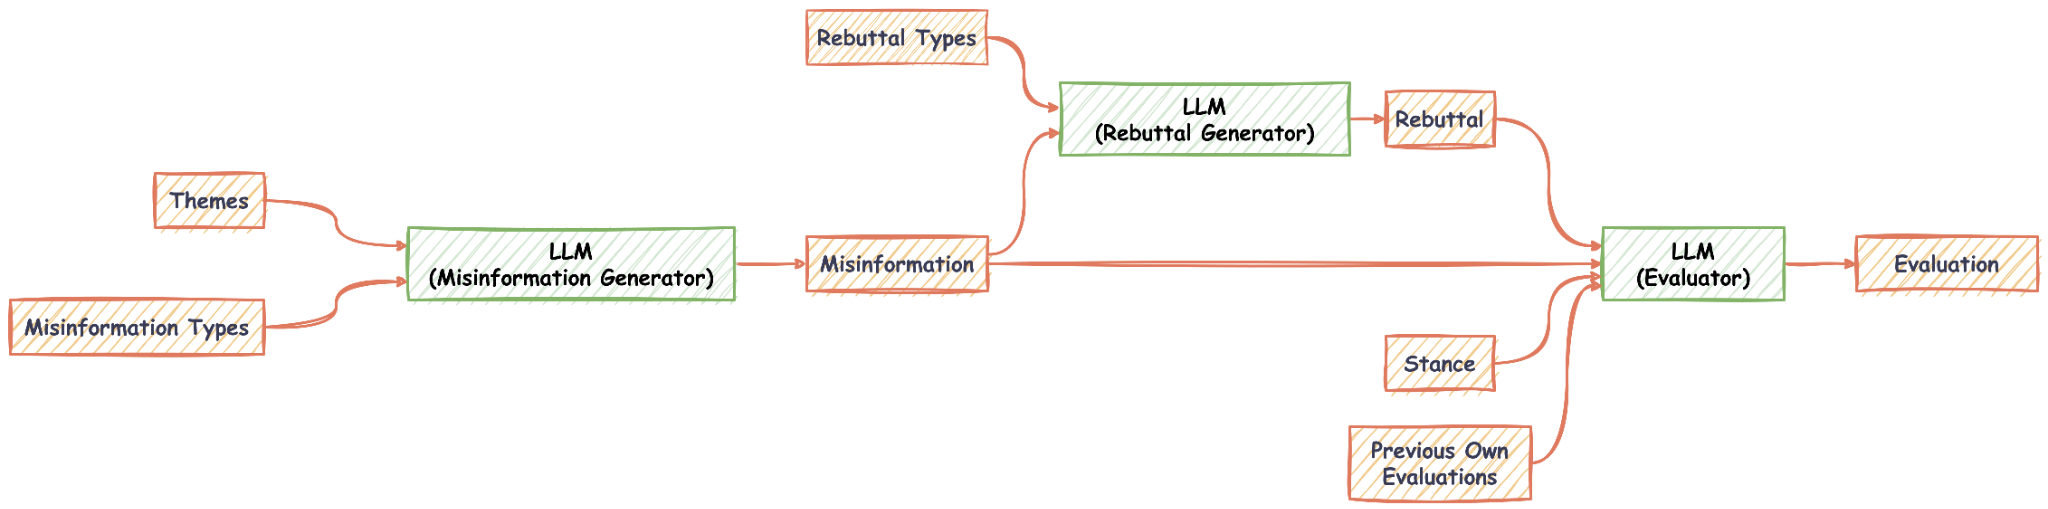
\includegraphics[width=\textwidth]{scheme.png}
    \caption{Research Scheme}
    \label{fig:scheme}
\end{figure*}

Despite these promising findings, we recognize limitations regarding the generalizability of our results. The chosen topic is inherently emotional and value-laden, and thus further research is necessary to determine if these findings hold for other less polarized or different contexts. Moreover, our evaluation agents are computational approximations of human judgments; future studies should validate these results through human-subject experiments.

Overall, our findings provide critical insights and practical guidelines for enhancing community-driven correction systems for Information Disorder like Community Notes. Additionally, they offer valuable implications for policymakers and platform administrators who aim to design more effective strategies to combat various forms of problematic information.

In the following sections, we detail our experimental design, analytic methodologies, and present in-depth analyses and discussions of our results, concluding with theoretical and practical implications.



\section{Method}
\subsection{Problem Formulation}
Formally, we construct a large-scale simulation environment utilizing Large Language Model (LLM)-based agents to represent individual evaluators on the platform X (formerly Twitter). Each evaluator agent traces the behavior of an actual user, remembering past Community Notes (CN) evaluations to inform subsequent judgments. Additionally, we prepare specialized Community Note-generating agents that simulate creators of Community Notes using ten distinct logical patterns derived from the Counter-Argument Logical Structure Analysis (CALSA) framework (Naito et al., 2024): Mitigation, Alternative, No Evidence, Another True Cause, Missing Mechanism \#1 and \#2, No Need to Address, Negative Effect Due to y, and Positive Effects of a Different Perspective from y (\#1 and \#2). The primary objective is to investigate how evaluator attributes and Community Note logical patterns influence evaluations.

The implementation of these agents leverages a modular agent design adapted from the User Modeling Track of the WWW'25 AgentSociety Challenge, employing Planning, Reasoning, Tool Use, and Memory modules (WWW'25 AgentSociety Challenge, 2025) to replicate realistic and strategic evaluation behaviors.

The implementation of agents is based on an adaptation of the User Modeling Track from the WWW'25 AgentSociety Challenge, which emphasizes modular agent designs comprising Planning, Reasoning, Tool Use, and Memory modules (WWW'25 AgentSociety Challenge, 2025). These modules facilitate realistic agent behavior, including strategic communication and evaluation tasks.

\section{Experiments}
In this experiment, we systematically evaluate the effectiveness of different rebuttal strategies against various types of misinformation across socially contentious topics. Our experimental design incorporates agent-based simulation to assess how different logical structures in rebuttals influence evaluation outcomes across diverse evaluator perspectives.

We selected "Gun Control" as our primary thematic domain, representing a socially significant and contentious topic with strong partisan dimensions. For this theme, we generated seven distinct categories of misinformation: Satire/parody, Misleading content, False connection, False context, Imposter content, Manipulated content, and Fabricated content. Each category represents a specific manifestation of misinformation as classified in contemporary misinformation research.

For each misinformation instance, we systematically generated ten different types of rebuttals based on the Counter-Argument Logical Structure Analysis (CALSA) framework (Naito et al., 2024). These rebuttal types include: Mitigation, Alternative, No Evidence, Another True Cause, Missing Mechanism (two variants), No Need to Address, Negative Effect Due to y, and Positive Effects of a Different Perspective from y (two variants). Each rebuttal type employs a distinct logical structure to counter the original misinformation.

To evaluate these rebuttals, we implemented two categories of evaluator agents: neutral agents and pro-misinformation agents, with five instances of each type. This design allows us to assess how rebuttals perform both with impartial evaluators and with those predisposed to accept the misinformation. Each agent evaluated rebuttals using a three-tier rating system ("helpful," "somewhat helpful," or "not helpful") accompanied by specific reasoning for their assessment.

Our experimental procedure consisted of three primary phases. The first phase involved misinformation generation using large language models to create realistic misinformation content for each category, ensuring they contained appropriate logical fallacies and appeared as authentic social media content. The second phase focused on rebuttal generation, where for each misinformation instance, we systematically applied the ten CALSA rebuttal strategies to create corresponding corrections. The final phase encompassed evaluation, wherein both neutral and pro-misinformation agents assessed each rebuttal, providing ratings and justifications based on their respective perspectives.



\section{Results}
Our analysis of the evaluation data revealed several significant patterns regarding the effectiveness of different rebuttal strategies across misinformation types and evaluator perspectives. The results are visualized through heatmaps that display the average helpfulness scores (on a scale of 0-2, where 2 represents "helpful") for each combination of misinformation type and rebuttal strategy.

\subsection{Topic-Specific Analysis}
\subsubsection{Gun Control Topic}
For the gun control topic, neutral evaluators showed distinct preferences for certain rebuttal strategies across misinformation types. The Satire/parody category received consistently high ratings (2.0) across almost all rebuttal strategies, suggesting that logical rebuttals are particularly effective against satirical misinformation. The Missing Mechanism 2 (MM2) strategy demonstrated remarkable effectiveness when addressing Fabricated content and False connection, consistently receiving high helpfulness scores. Similarly, the Negative Effect (Neg eff) strategy proved highly effective against multiple misinformation types.

In contrast, pro-misinformation evaluators exhibited markedly different response patterns for gun control content. These evaluators generally assigned lower helpfulness ratings across most rebuttal strategies, particularly for the Diff Per1 strategy, which received notably low scores across multiple misinformation types. However, interestingly, the Missing Mechanism strategies maintained relatively high effectiveness even among pro-misinformation evaluators, especially when addressing Fabricated content and Misleading content.

\subsubsection{Abortion Ban Topic}
For abortion-related misinformation, neutral evaluators showed a more varied response pattern compared to the gun control topic. The Fabricated content category showed high effectiveness for MM2 strategy (2.0), while False connection misinformation was most effectively countered using the Neg eff strategy (2.0). Notably, False context misinformation proved particularly resistant to correction, with most strategies receiving moderate ratings.

Pro-misinformation evaluators assessing abortion-related content showed strong resistance to most rebuttal strategies, with particularly low ratings for evidence-based approaches (Diff Per1, Neg eff) when addressing Fabricated content and False context. This suggests that on highly polarized topics like abortion, factual corrections may be less persuasive to those predisposed to accept misinformation. However, the Alt strategy showed unexpected effectiveness with pro-misinformation evaluators when addressing several misinformation types, indicating that offering alternative explanations may be more acceptable than direct contradiction.

\subsubsection{Partisan Alignment Topic}
For partisan alignment misinformation, neutral evaluators showed strong positive responses to rebuttals addressing Fabricated content, particularly using ATC, MM1, and No Evidence strategies. Imposter content was also effectively countered using MM1 and Mig strategies. This suggests that for politically charged content, addressing the underlying mechanisms and providing alternative true causes is particularly effective with neutral audiences.

Pro-misinformation evaluators showed the strongest resistance to corrections in this topic area, with notably low ratings across multiple strategies, particularly for Manipulated content. This indicates that partisan-aligned misinformation may be the most difficult to correct among those predisposed to accept it. However, the MM1 strategy maintained moderate effectiveness even with these evaluators, suggesting its potential as a broadly acceptable approach for politically charged misinformation.

\subsection{Cross-Topic Analysis}

Our cross-topic analysis revealed several consistent patterns in rebuttal effectiveness. Across all three topics, the Missing Mechanism strategies (MM1 and MM2) demonstrated the most consistent effectiveness, particularly with neutral evaluators. This suggests that addressing the logical structure of misinformation may be more persuasive than simply providing contradictory evidence.

The effectiveness of rebuttal strategies varied significantly by misinformation type across topics. Fabricated content was generally most susceptible to correction with neutral evaluators, while Manipulated content and False context proved more resistant. With pro-misinformation evaluators, Satire/parody was most effectively countered across topics, while Imposter content and Fabricated content showed the strongest resistance to correction.

Notably, the polarization between neutral and pro-misinformation evaluations was most pronounced for the Partisan Alignment topic, followed by Abortion Ban, with Gun Control showing the least polarization. This aligns with the relative political polarization of these topics in contemporary discourse.

\subsection{Polarization Analysis}

The polarization analysis further illuminated the divergence in evaluations between neutral and pro-misinformation agents across topics. The No Evidence and Negative Effect strategies exhibited the highest polarization across all topics, with neutral evaluators finding them substantially more helpful than pro-misinformation evaluators. This suggests that directly challenging evidence or highlighting negative consequences tends to reinforce rather than reduce polarization.

Conversely, the Missing Mechanism 1 and Alternative strategies demonstrated the least polarization across topics, suggesting their potential utility as broadly acceptable rebuttal approaches across different audience perspectives. This finding has significant implications for designing correction strategies aimed at diverse audiences.

\begin{figure*}
\centering
\begin{subfigure}{0.28\textwidth}
    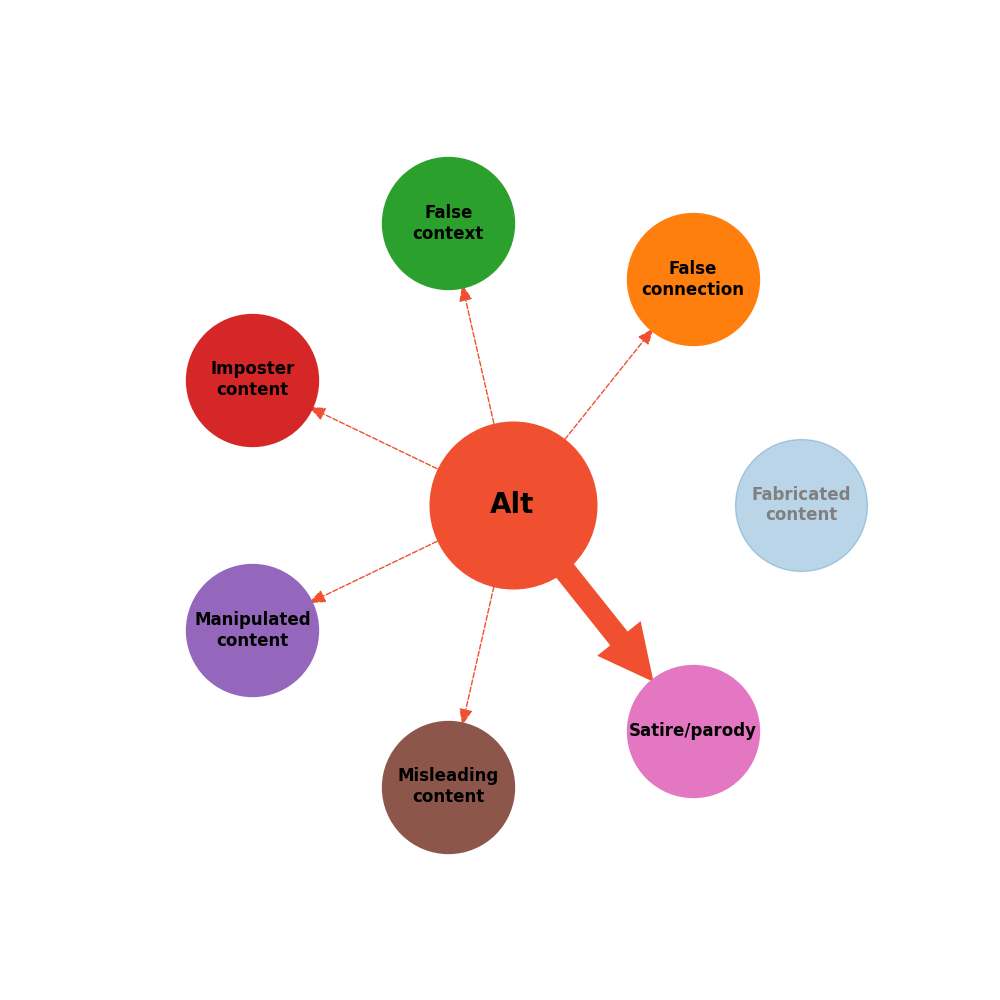
\includegraphics[width=\textwidth]{rebuttal_Alt.png}
    \caption{Alternative}
    \label{fig:rebuttal_alt}
\end{subfigure}
\hfill
\begin{subfigure}{0.28\textwidth}
    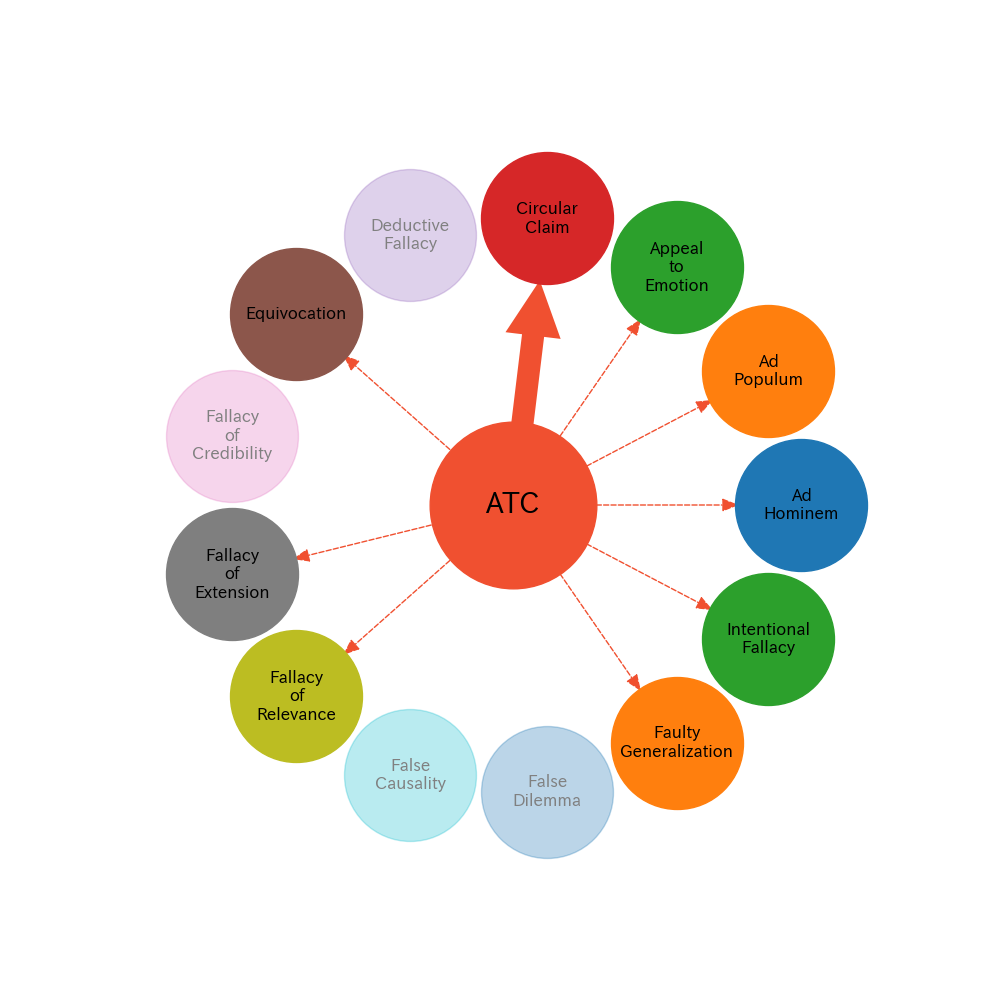
\includegraphics[width=\textwidth]{rebuttal_ATC.png}
    \caption{Another True Cause}
    \label{fig:rebuttal_atc}
\end{subfigure}
\hfill
\begin{subfigure}{0.28\textwidth}
    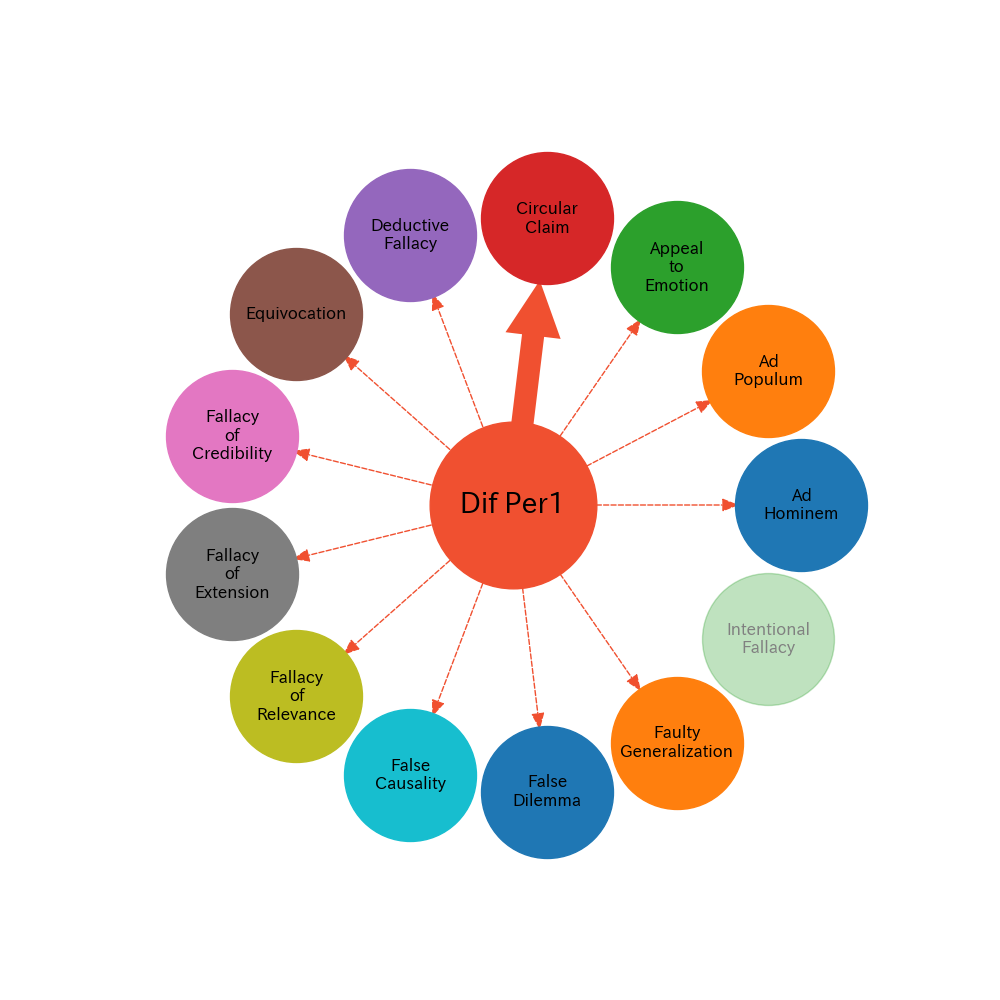
\includegraphics[width=\textwidth]{rebuttal_Dif_Per1.png}
    \caption{Different Perspective 1}
    \label{fig:rebuttal_diffper1}
\end{subfigure}

\begin{subfigure}{0.28\textwidth}
    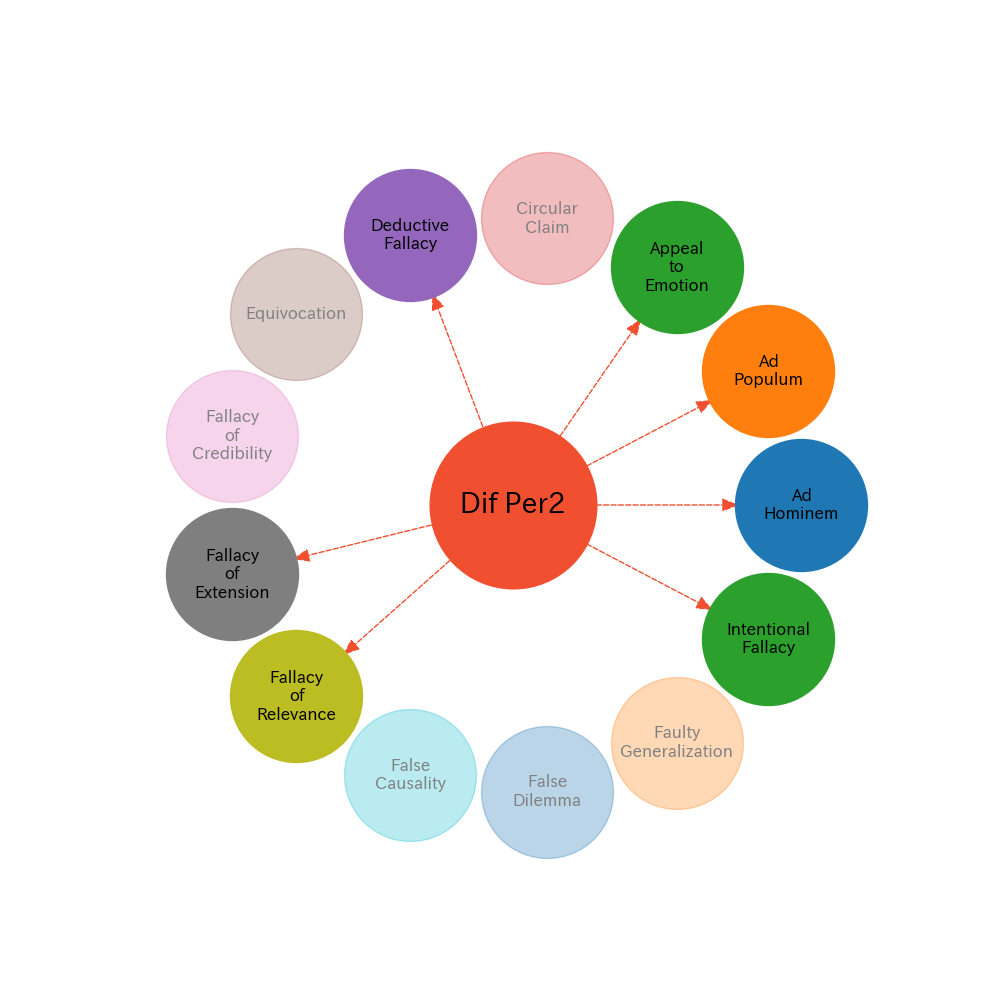
\includegraphics[width=\textwidth]{rebuttal_Dif_Per2.png}
    \caption{Different Perspective 2}
    \label{fig:rebuttal_diffper2}
\end{subfigure}
\hfill
\begin{subfigure}{0.28\textwidth}
    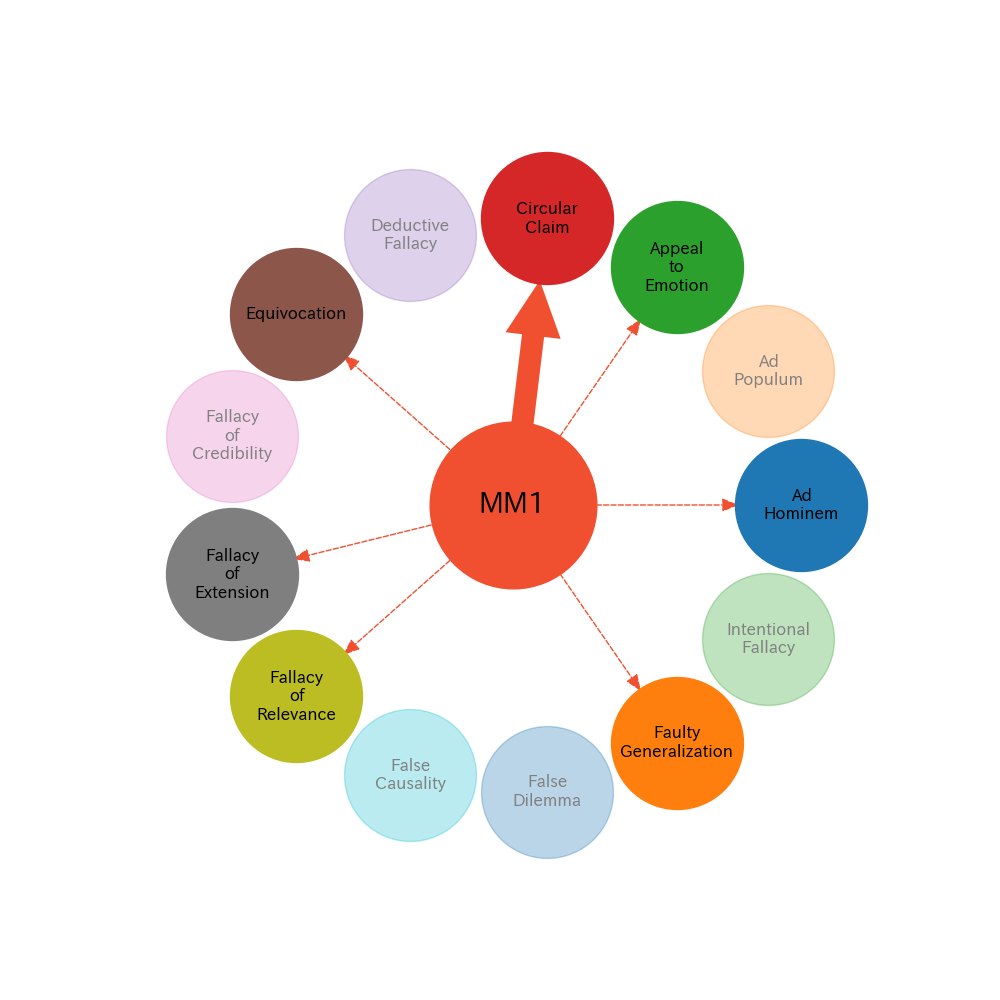
\includegraphics[width=\textwidth]{rebuttal_MM1.png}
    \caption{Missing Mechanism 1}
    \label{fig:rebuttal_mm1}
\end{subfigure}
\hfill
\begin{subfigure}{0.28\textwidth}
    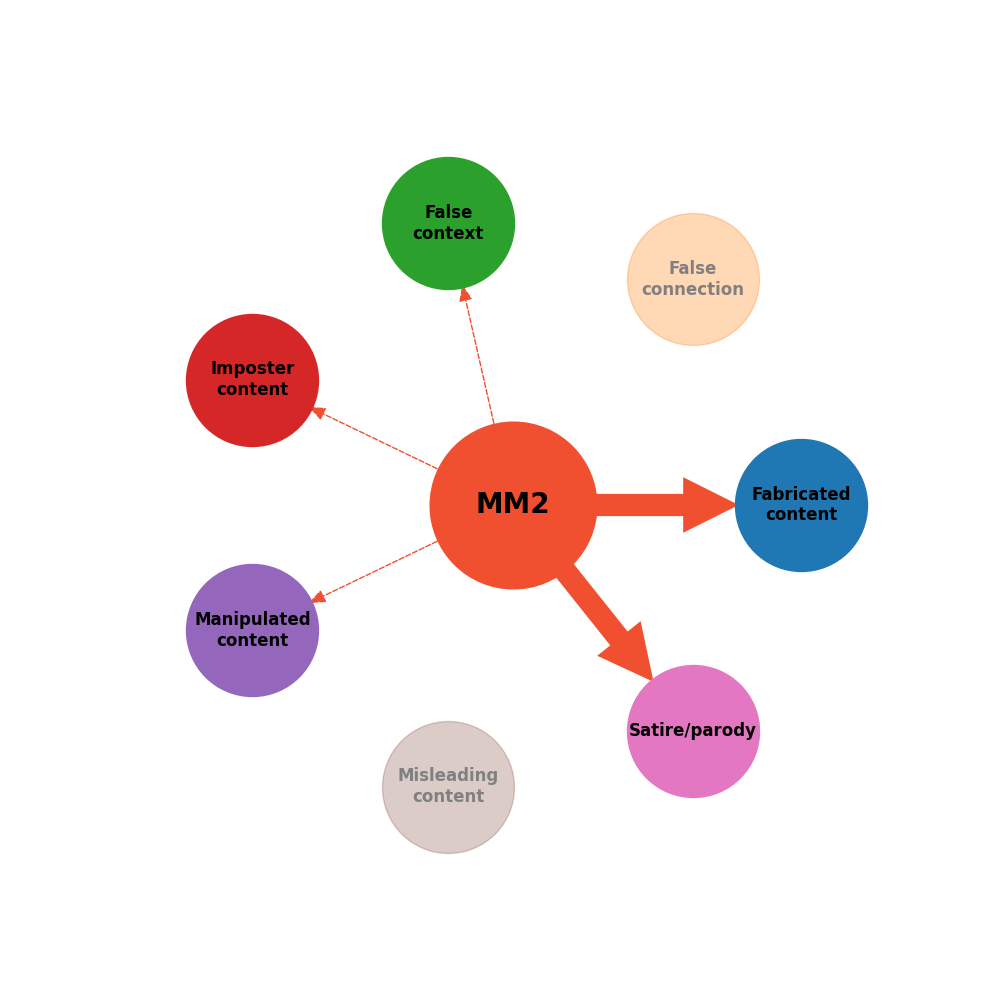
\includegraphics[width=\textwidth]{rebuttal_MM2.png}
    \caption{Missing Mechanism 2}
    \label{fig:rebuttal_mm2}
\end{subfigure}

\begin{subfigure}{0.28\textwidth}
    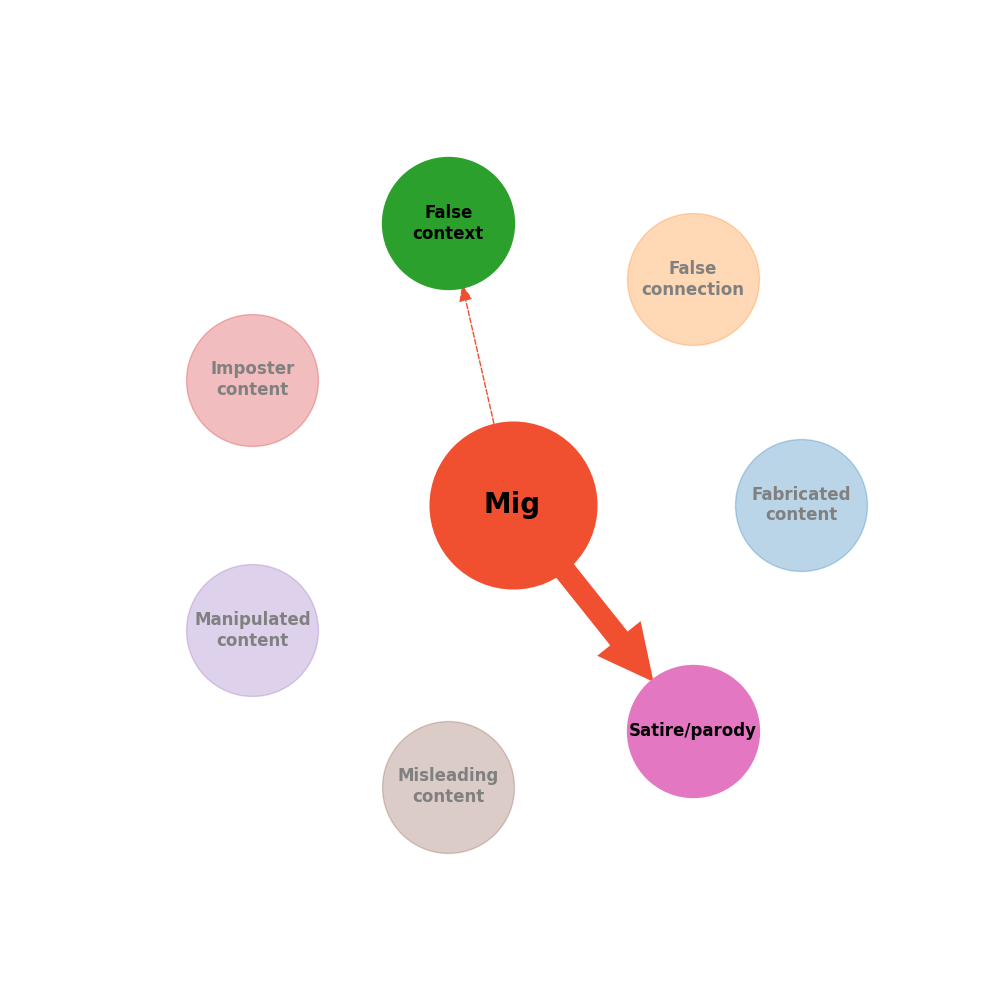
\includegraphics[width=\textwidth]{rebuttal_Mig.png}
    \caption{Mitigation}
    \label{fig:rebuttal_mig}
\end{subfigure}
\hfill
\begin{subfigure}{0.28\textwidth}
    \includegraphics[width=\textwidth]{rebuttal_Neg_Eff.png}
    \caption{Negative Effect}
    \label{fig:rebuttal_negeff}
\end{subfigure}
\hfill
\begin{subfigure}{0.28\textwidth}
    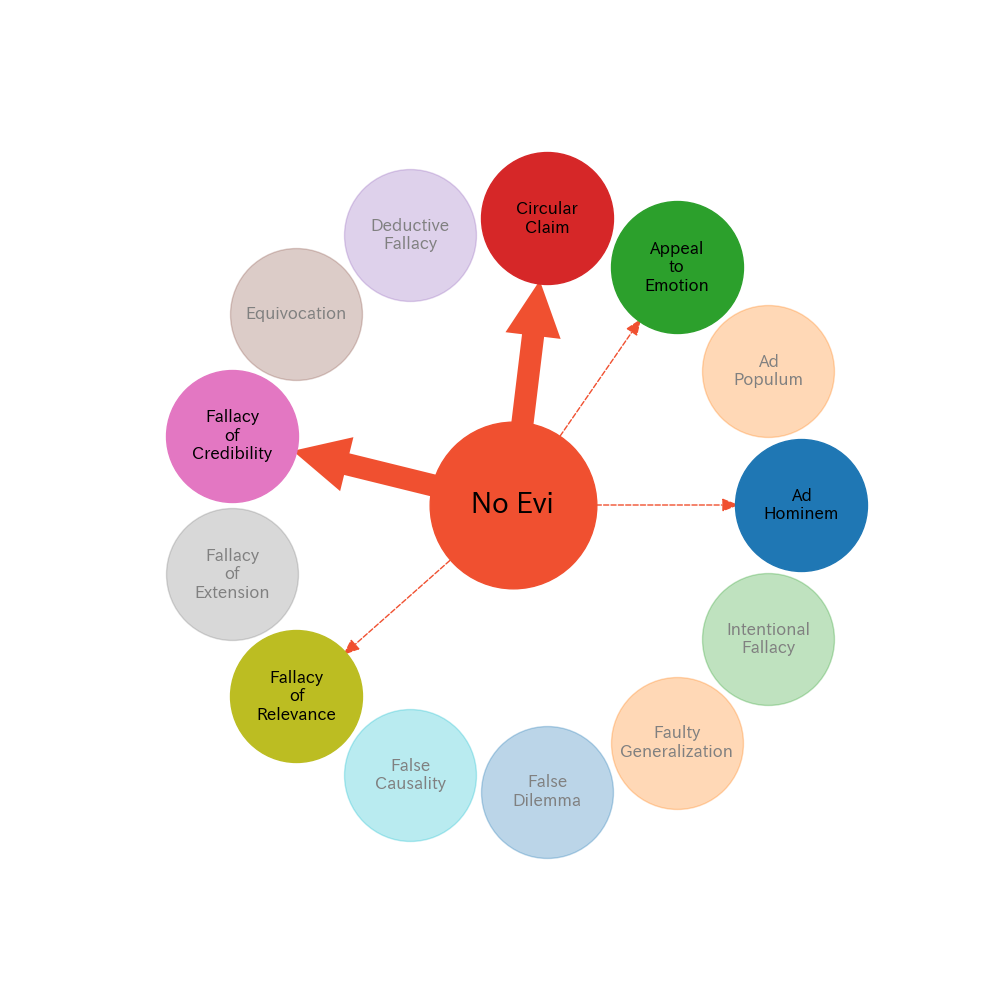
\includegraphics[width=\textwidth]{rebuttal_No_Evi.png}
    \caption{No Evidence}
    \label{fig:rebuttal_noevi}
\end{subfigure}

\begin{subfigure}{0.28\textwidth}
    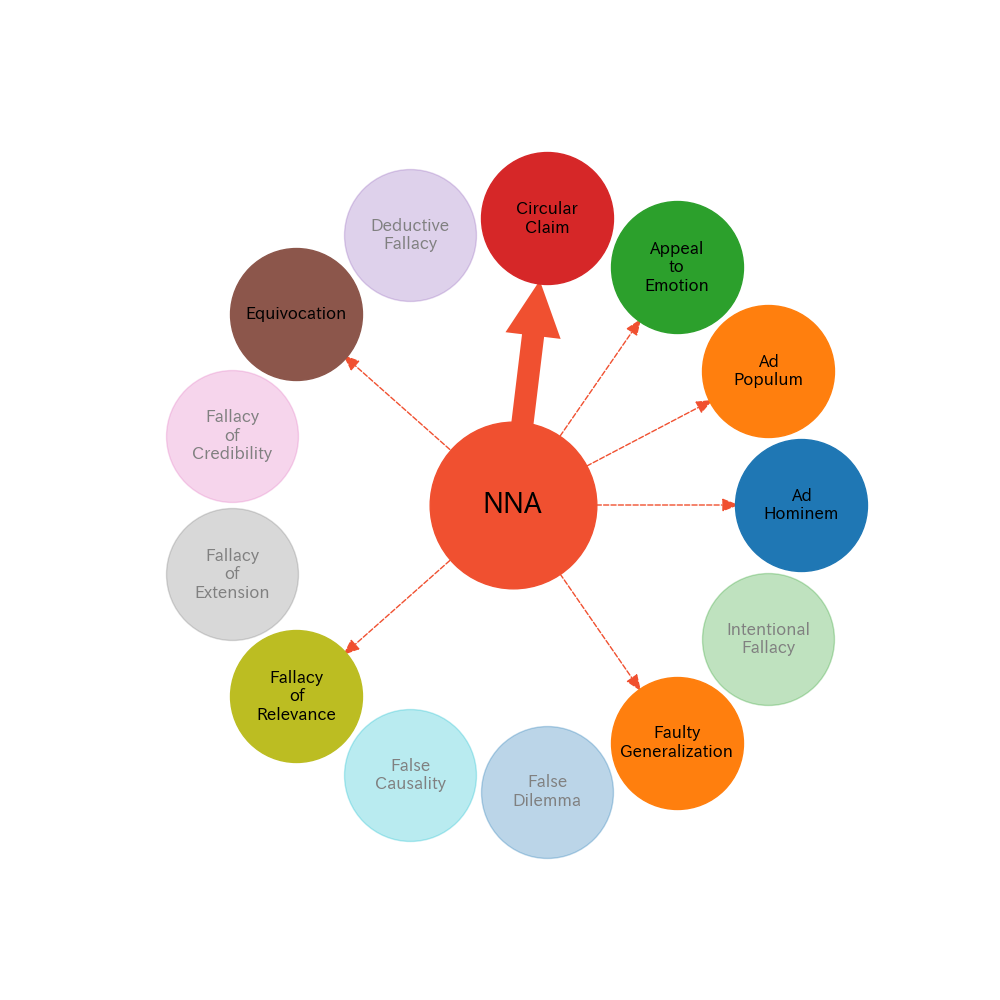
\includegraphics[width=\textwidth]{rebuttal_NNA.png}
    \caption{No Need to Address}
    \label{fig:rebuttal_noneed}
\end{subfigure}

\caption{Effectiveness of Different Rebuttal Strategies}
\label{fig:rebuttals_combined}
\end{figure*}

These findings highlight the complex interplay between misinformation types, rebuttal strategies, topic sensitivity, and evaluator predispositions. While certain strategies like Missing Mechanism demonstrate broad effectiveness across evaluator types and topics, others appear to trigger resistance among those predisposed to accept misinformation, particularly on highly polarized topics. This suggests that the optimal selection of rebuttal strategies should consider not only the type of misinformation being addressed but also the topic context and the likely predispositions of the target audience.

\section{Discussion}
Building on our results, we can draw several important conclusions about the effectiveness of logical rebuttal strategies against misinformation. First, our findings demonstrate that the effectiveness of rebuttals is not uniform but varies significantly based on the interaction between misinformation type, rebuttal strategy, topic context, and audience predisposition.

The consistent effectiveness of the Missing Mechanism strategies across different topics and evaluator types suggests that addressing the logical structure of misinformation may be more persuasive than simply providing contradictory evidence. By explaining why the causal or logical connections in misinformation are flawed, these strategies appear to bypass some of the resistance typically encountered with more direct factual corrections.

The topic-specific variations in rebuttal effectiveness highlight the importance of contextual factors in misinformation correction. For highly polarized topics like abortion and partisan alignment, we observed stronger resistance to correction among pro-misinformation evaluators compared to the relatively less polarized gun control topic. This suggests that correction strategies may need to be tailored not only to misinformation types but also to topic sensitivity.

The polarization analysis provides particularly valuable insights for practical applications. Strategies that minimize polarization, such as Missing Mechanism 1 and Alternative, may be preferable in contexts where reaching diverse audiences is prioritized. Conversely, strategies that maximize effectiveness with neutral audiences but increase polarization, such as No Evidence and Negative Effect, may be more appropriate when the primary goal is to prevent neutral individuals from adopting misinformation rather than changing the minds of those already convinced.

These findings have significant implications for the design of community-driven correction systems like Community Notes. Platform designers might consider implementing recommendation systems that suggest optimal rebuttal strategies based on misinformation type and topic context. Additionally, training materials for community note contributors could emphasize the effectiveness of explaining missing mechanisms and providing alternatives rather than simply contradicting claims or highlighting lack of evidence.

\section{Limitations and Future Work}
While our study provides valuable insights into rebuttal effectiveness, several limitations should be acknowledged. First, our agent-based simulation approach, while allowing for systematic evaluation across multiple conditions, may not fully capture the complexity of human responses to misinformation and corrections. Future work should validate these findings through human-subject experiments.

Second, our study focused on three specific topics, which, while diverse, cannot represent the full spectrum of misinformation contexts. Additional research is needed to determine whether these patterns hold across other domains such as health misinformation, scientific misinformation, or conspiracy theories.

Third, our binary categorization of evaluators as either neutral or pro-misinformation represents a simplification of the complex spectrum of audience predispositions. Future studies should explore more nuanced audience models, including varying degrees of prior belief and different motivational factors.

Finally, our study evaluated immediate responses to rebuttals but did not assess long-term persuasive effects. Longitudinal studies examining how different rebuttal strategies influence beliefs over time would provide valuable complementary insights.

\section{Conclusion}
Our study provides empirical evidence for the differential effectiveness of logical rebuttal strategies against various types of misinformation across different topics and audience predispositions. The findings highlight the particular effectiveness of strategies that address missing mechanisms in logical arguments and offer alternatives to misinformation claims, especially when communicating with diverse audiences.

These insights contribute to both theoretical understanding of misinformation correction and practical applications for community-driven correction systems. By tailoring rebuttal strategies to misinformation types, topic contexts, and audience characteristics, correction efforts can potentially achieve greater effectiveness while minimizing polarization.

As misinformation continues to pose significant challenges to public discourse and decision-making, evidence-based approaches to correction become increasingly vital. Our findings offer a foundation for more sophisticated and contextually sensitive correction strategies that can help communities collectively navigate the complex information landscape of contemporary digital media.


\end{document}